% Options for packages loaded elsewhere
\PassOptionsToPackage{unicode}{hyperref}
\PassOptionsToPackage{hyphens}{url}
\documentclass[
]{article}
\usepackage{xcolor}
\usepackage{amsmath,amssymb}
\setcounter{secnumdepth}{-\maxdimen} % remove section numbering
\usepackage{iftex}
\ifPDFTeX
  \usepackage[T1]{fontenc}
  \usepackage[utf8]{inputenc}
  \usepackage{textcomp} % provide euro and other symbols
\else % if luatex or xetex
  \usepackage{unicode-math} % this also loads fontspec
  \defaultfontfeatures{Scale=MatchLowercase}
  \defaultfontfeatures[\rmfamily]{Ligatures=TeX,Scale=1}
\fi
\usepackage{lmodern}
\ifPDFTeX\else
  % xetex/luatex font selection
\fi
% Use upquote if available, for straight quotes in verbatim environments
\IfFileExists{upquote.sty}{\usepackage{upquote}}{}
\IfFileExists{microtype.sty}{% use microtype if available
  \usepackage[]{microtype}
  \UseMicrotypeSet[protrusion]{basicmath} % disable protrusion for tt fonts
}{}
\makeatletter
\@ifundefined{KOMAClassName}{% if non-KOMA class
  \IfFileExists{parskip.sty}{%
    \usepackage{parskip}
  }{% else
    \setlength{\parindent}{0pt}
    \setlength{\parskip}{6pt plus 2pt minus 1pt}}
}{% if KOMA class
  \KOMAoptions{parskip=half}}
\makeatother
\usepackage{color}
\usepackage{fancyvrb}
\newcommand{\VerbBar}{|}
\newcommand{\VERB}{\Verb[commandchars=\\\{\}]}
\DefineVerbatimEnvironment{Highlighting}{Verbatim}{commandchars=\\\{\}}
% Add ',fontsize=\small' for more characters per line
\newenvironment{Shaded}{}{}
\newcommand{\AlertTok}[1]{\textcolor[rgb]{1.00,0.00,0.00}{\textbf{#1}}}
\newcommand{\AnnotationTok}[1]{\textcolor[rgb]{0.38,0.63,0.69}{\textbf{\textit{#1}}}}
\newcommand{\AttributeTok}[1]{\textcolor[rgb]{0.49,0.56,0.16}{#1}}
\newcommand{\BaseNTok}[1]{\textcolor[rgb]{0.25,0.63,0.44}{#1}}
\newcommand{\BuiltInTok}[1]{\textcolor[rgb]{0.00,0.50,0.00}{#1}}
\newcommand{\CharTok}[1]{\textcolor[rgb]{0.25,0.44,0.63}{#1}}
\newcommand{\CommentTok}[1]{\textcolor[rgb]{0.38,0.63,0.69}{\textit{#1}}}
\newcommand{\CommentVarTok}[1]{\textcolor[rgb]{0.38,0.63,0.69}{\textbf{\textit{#1}}}}
\newcommand{\ConstantTok}[1]{\textcolor[rgb]{0.53,0.00,0.00}{#1}}
\newcommand{\ControlFlowTok}[1]{\textcolor[rgb]{0.00,0.44,0.13}{\textbf{#1}}}
\newcommand{\DataTypeTok}[1]{\textcolor[rgb]{0.56,0.13,0.00}{#1}}
\newcommand{\DecValTok}[1]{\textcolor[rgb]{0.25,0.63,0.44}{#1}}
\newcommand{\DocumentationTok}[1]{\textcolor[rgb]{0.73,0.13,0.13}{\textit{#1}}}
\newcommand{\ErrorTok}[1]{\textcolor[rgb]{1.00,0.00,0.00}{\textbf{#1}}}
\newcommand{\ExtensionTok}[1]{#1}
\newcommand{\FloatTok}[1]{\textcolor[rgb]{0.25,0.63,0.44}{#1}}
\newcommand{\FunctionTok}[1]{\textcolor[rgb]{0.02,0.16,0.49}{#1}}
\newcommand{\ImportTok}[1]{\textcolor[rgb]{0.00,0.50,0.00}{\textbf{#1}}}
\newcommand{\InformationTok}[1]{\textcolor[rgb]{0.38,0.63,0.69}{\textbf{\textit{#1}}}}
\newcommand{\KeywordTok}[1]{\textcolor[rgb]{0.00,0.44,0.13}{\textbf{#1}}}
\newcommand{\NormalTok}[1]{#1}
\newcommand{\OperatorTok}[1]{\textcolor[rgb]{0.40,0.40,0.40}{#1}}
\newcommand{\OtherTok}[1]{\textcolor[rgb]{0.00,0.44,0.13}{#1}}
\newcommand{\PreprocessorTok}[1]{\textcolor[rgb]{0.74,0.48,0.00}{#1}}
\newcommand{\RegionMarkerTok}[1]{#1}
\newcommand{\SpecialCharTok}[1]{\textcolor[rgb]{0.25,0.44,0.63}{#1}}
\newcommand{\SpecialStringTok}[1]{\textcolor[rgb]{0.73,0.40,0.53}{#1}}
\newcommand{\StringTok}[1]{\textcolor[rgb]{0.25,0.44,0.63}{#1}}
\newcommand{\VariableTok}[1]{\textcolor[rgb]{0.10,0.09,0.49}{#1}}
\newcommand{\VerbatimStringTok}[1]{\textcolor[rgb]{0.25,0.44,0.63}{#1}}
\newcommand{\WarningTok}[1]{\textcolor[rgb]{0.38,0.63,0.69}{\textbf{\textit{#1}}}}
\usepackage{graphicx}
\makeatletter
\newsavebox\pandoc@box
\newcommand*\pandocbounded[1]{% scales image to fit in text height/width
  \sbox\pandoc@box{#1}%
  \Gscale@div\@tempa{\textheight}{\dimexpr\ht\pandoc@box+\dp\pandoc@box\relax}%
  \Gscale@div\@tempb{\linewidth}{\wd\pandoc@box}%
  \ifdim\@tempb\p@<\@tempa\p@\let\@tempa\@tempb\fi% select the smaller of both
  \ifdim\@tempa\p@<\p@\scalebox{\@tempa}{\usebox\pandoc@box}%
  \else\usebox{\pandoc@box}%
  \fi%
}
% Set default figure placement to htbp
\def\fps@figure{htbp}
\makeatother
\setlength{\emergencystretch}{3em} % prevent overfull lines
\providecommand{\tightlist}{%
  \setlength{\itemsep}{0pt}\setlength{\parskip}{0pt}}
\usepackage{bookmark}
\IfFileExists{xurl.sty}{\usepackage{xurl}}{} % add URL line breaks if available
\urlstyle{same}
\hypersetup{
  pdftitle={Relazione del progetto d'esame di Editoria Digitale},
  pdfauthor={Salvatore Torrisi matricola 10451A},
  hidelinks,
  pdfcreator={LaTeX via pandoc}}

\title{Relazione del progetto d'esame di Editoria Digitale}
\author{Salvatore Torrisi matricola 10451A}
\date{a.a. 2024/2025}

\begin{document}
\maketitle

\begin{figure}
\centering

\includegraphics[width=1.04167in,height=\textheight,keepaspectratio]{./foto/minerva.jpg}
\caption{Logo UNIMI}
\end{figure}

\section{Agire per il Futuro: Guida alla
Sostenibilità}\label{agire-per-il-futuro-guida-alla-sostenibilituxe0}

\begin{itemize}
\tightlist
\item
  \href{www.google.com}{Link al poster}
\item
  \href{www.google.com}{Link alla repository}
\end{itemize}

\subsection{Introduzione}\label{introduzione}

Il progetto ``Agire per il Futuro: Guida alla Sostenibilità'' è stato
sviluppato per conto di un ente no-profit che promuove la sostenibilità
ambientale. L'obiettivo principale è sensibilizzare i giovani di età
compresa tra i 18 e i 25 anni sui temi del cambiamento climatico e
dell'impatto ambientale delle scelte quotidiane. Il prodotto editoriale
ideato è un poster promozionale distribuito tramite le storie Instagram
dell'ente, con adesivi per il download diretto.

\subsection{Ideazione}\label{ideazione}

\subsubsection{Tema}\label{tema}

Il tema centrale del progetto è il cambiamento climatico e l'importanza
di comportamenti sostenibili. Sono state approfondite le principali
problematiche ambientali, come l'aumento delle emissioni di CO2, l'uso
eccessivo delle risorse naturali e l'inquinamento, evidenziando domande
frequenti e bisogni insoddisfatti del pubblico giovane. Oltre a ciò,
l'ente tiene a realizzare delle iniziative per i giovani per combattere
il cambiamento climatico, e tramite questo progetto editoriale vuole far
diffondere sempre di più la voce su queste attività.

\subsubsection{Destinatari}\label{destinatari}

Il target è rappresentato da giovani adulti (18-25 anni), digitalmente
competenti e attivi sui social media. Attraverso la tecnica delle
personas, è stato immaginato un pubblico interessato a comprendere
meglio come contribuire alla sostenibilità ambientale. Ad esempio, una
persona fittizia, Anna, 22 anni, studentessa universitaria di scienze
ambientali, utilizza spesso Instagram per condividere e scoprire
contenuti legati alla sostenibilità. Anna cerca suggerimenti pratici su
come ridurre il proprio impatto ambientale e è interessata a iniziative
locali sul tema. Un'altra persona, Marco, 24 anni, sviluppatore web, è
interessato a tecnologie verdi e vuole adottare stili di vita
sostenibili. Entrambi rappresentano target chiave del progetto e
riflettono le diverse esigenze del pubblico giovane. e desideroso di
informazioni pratiche e accessibili.

\subsubsection{Modello di fruizione}\label{modello-di-fruizione}

Il poster è pensato per una fruizione digitale semplice ed efficace,
tramite un semplice PDF visualizzabile da mobile. Nel poster viene
utilizzato un linguaggio chiaro e diretto, integrato di immagini per
catturare l'attenzione.

La parte centrale del poster è stata strutturata per accogliere
aggiornamenti regolari con notizie e iniziative legate al cambiamento
climatico.

\subsubsection{Canali di distribuzione}\label{canali-di-distribuzione}

Il principale canale di distribuzione è Instagram, utilizzando storie
con adesivi per il download. Il formato scelto è PDF per garantire
compatibilità e alta qualità visiva. Il design è orientato verso uno
stile informale ma professionale, capace di comunicare efficacemente il
messaggio dell'ente.

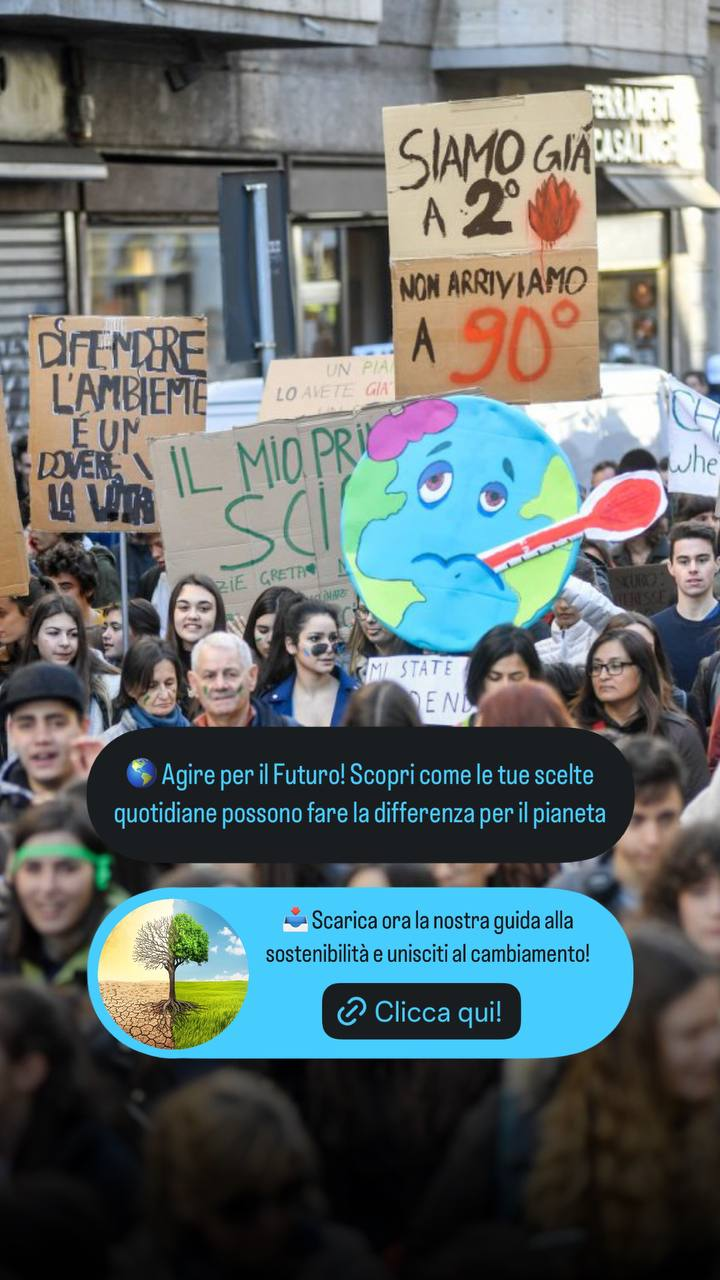
\includegraphics[width=\linewidth,height=2.60417in,keepaspectratio]{./foto/insta.jpg}
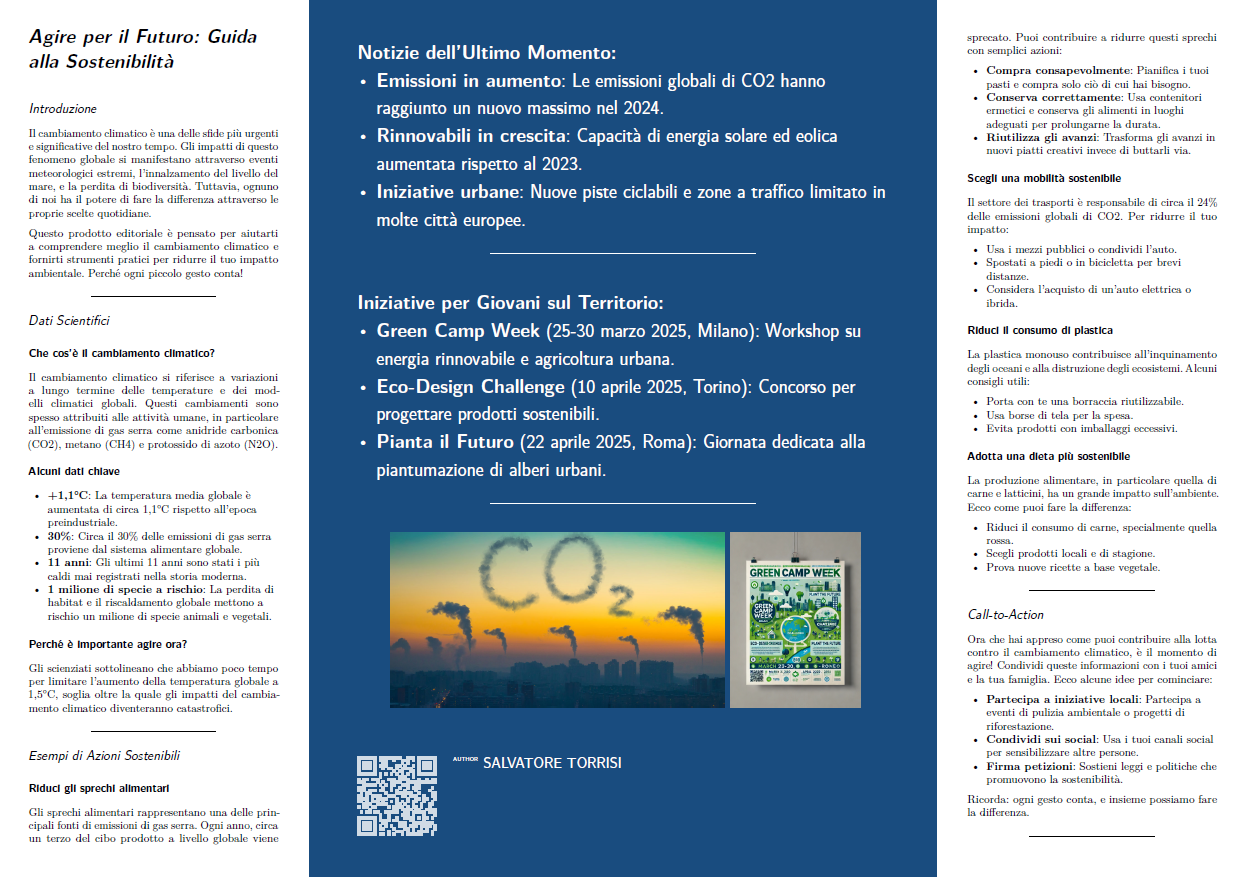
\includegraphics[width=\linewidth,height=2.60417in,keepaspectratio]{./foto/progetto.jpg}

\subsection{Processo di Produzione}\label{processo-di-produzione}

\subsubsection{Acquisizione dei
contenuti}\label{acquisizione-dei-contenuti}

I contenuti sono stati generati con l'ausilio di ChatGPT, applicando
tecniche di prompt engineering per ottenere testi scientificamente
accurati e adatti al target. Per le immagini sono state utilizzate fonti
libere per minimizzare i costi di acquisizione.

\subsubsection{Gestione documentale}\label{gestione-documentale}

Il flusso documentale comprende: 1. Raccolta dei contenuti tramite
prompt engineering con ChatGPT. 2. Scrittura del contenuto in Markdown
per garantire flessibilità e aggiornabilità. 3. Conversione in LaTeX
tramite Pandoc, utilizzando il template ``ANT Center Poster''. 4.
Controllo e approvazione del layout e dei contenuti.

\begin{Shaded}
\begin{Highlighting}[]
\NormalTok{graph LR}
\NormalTok{A[Scrittura Markdown] {-}{-}\textgreater{} B[Conversione in LaTeX]}
\NormalTok{B {-}{-}\textgreater{} C[Personalizzazione Template]}
\NormalTok{C {-}{-}\textgreater{} D[Distribuzione]}
\end{Highlighting}
\end{Shaded}

\subsubsection{Tecnologie adottate}\label{tecnologie-adottate}

\begin{itemize}
\tightlist
\item
  \textbf{Markdown}: Per la creazione e la gestione dei contenuti.
\item
  \textbf{Pandoc}: Per la conversione in LaTeX e l'applicazione del
  template.
\item
  \textbf{LaTeX}: Per la generazione del poster.
\end{itemize}

\subsubsection{Esecuzione del flusso}\label{esecuzione-del-flusso}

Il flusso di produzione è completamente documentato e riproducibile
attraverso i comandi e le configurazioni forniti. Il comando utilizzato
per la conversione principale è:

\begin{verbatim}
pandoc -s contenuto.md -o output.tex -V documentclass=antposter
\end{verbatim}

\subsection{Valutazione dei risultati
raggiunti}\label{valutazione-dei-risultati-raggiunti}

\subsubsection{Valutazione del flusso di
produzione}\label{valutazione-del-flusso-di-produzione}

Il flusso ha permesso di: ?

\subsubsection{Confronto con lo stato
dell'arte}\label{confronto-con-lo-stato-dellarte}

Rispetto ai metodi tradizionali, l'approccio adottato ha reso il
processo più efficiente e innovativo, grazie alla flessibilità offerta
da Markdown e Pandoc.

\subsubsection{Limiti emersi}\label{limiti-emersi}

\begin{itemize}
\tightlist
\item
  Difficoltà iniziale nell'adattare il template LaTeX alle esigenze
  specifiche del progetto.
\item
  Limitazioni nella gestione degli spazi e delle configurazioni avanzate
  del template.
\end{itemize}

\subsection{Conclusioni}\label{conclusioni}

Il progetto ha raggiunto gli obiettivi prefissati, sensibilizzando il
target giovane con un prodotto editoriale digitale coinvolgente e
aggiornabile. I risultati più soddisfacenti riguardano la qualità visiva
del poster e l'efficacia del flusso di produzione. Tuttavia, rimangono
margini di miglioramento nella personalizzazione dei template.

\subsection{Bibliografia e sitografia}\label{bibliografia-e-sitografia}

Elenco delle fonti principali: -
\href{https://www.overleaf.com/gallery/tagged/poster}{ANT Center Poster
Template} - Fonti scientifiche e articoli generati tramite ChatGPT.

\end{document}
